\section{Proper orthogonal decomposition}
\label{sec:POD}

{The proper orthogonal decomposition (POD) is a robust method identifying high-energy coherent structures in spatio-temporal data. Consequently, POD is often applied in the fields of turbulence analysis \citep{uruba2020,taira2020} and modeling \citep{gatski1991,shinde2020}. As a purely data-driven technique, it can be readily used to analyze both experimental and numerical data.}

%~ One of the possible applications of the proper orthogonal decomposition (POD) lies in identification of high-energy coherent structures in spatio-temporal data. Consequently, POD is often applied in the fields of turbulence analysis \citep{uruba2020,taira2020} and modeling \citep{gatski1991,shinde2020}. Simultaneously, POD is a purely data-driven and robust method and as such, it can be readily used to analyze both experimental and numerical data.


% \noteMI{====ONLY COPY-PASTE=====}

Both the experimental and simulation data are generated by sampling the studied system at given times,
\begin{equation}
\label{eq:snapshots}
    \bm{S} = \left\{\bm{y}_{j}:=\bm{y}(t_{j}) \right\}_{j=1}^{n}\,,\quad t_{j}\in (0,T]\,,
\end{equation}
where $\bm{S}$ is a set of system \textit{snapshots} and $\bm{y}_{j}$ is the vector of data at time $t_{j}$.

If all the system snapshots have the same dimension, i.e. $\bm{y}_{j}\in\mathbb{R}^{m}\,,j=1,\dots,n$, the set $\bm{S}$ may be rearranged into the matrix of snapshots
\begin{equation}
\label{eq:matrixOfSnapshots}
    Y = \left[\bm{y}_{1},\dots,\bm{y}_{n}\right] \in \mathbb{R}^{m\times n}\,,\quad \mathrm{rank}\,(Y) = n\,\,
\end{equation}
where we assumed that the number of system snapshots $n$ is lower than the data dimension $m$, which is commonly true for both the experimental and numerical data.

The standard POD algorithms are based on the singular value decomposition (SVD) of the matrix $Y$. 
\begin{equation}
\label{eq:svdY}
\begin{array}{*1{>{\displaystyle}c}}
    Y = \Psi \Sigma \Phi^{\transp}\,,\Psi \in \mathbb{R}^{m\times m}, \Phi\in\mathbb{R}^{n\times n}, \Sigma = \mathrm{diag}\,(\sigma_{1},\dots,\sigma_{m}) \in \mathbb{R}^{m\times n}\\[0.3cm]
    \Psi\Psi^{\transp} = E_{m}\,,\,\Phi\Phi^{T} = E_{n}\,,\,\sigma_{1}\geq\sigma_{2}\geq\dots\geq\sigma_{n} > 0 = \sigma_{n+1} = \dots = \sigma_{m}
\end{array}    
\end{equation}
where $E_{m}$ and $E_{n}$ are identity matrices in $\mathbb{R}^{m\times m}$ and $\mathbb{R}^{n\times n}$, respectively, and the first $n$ columns of the matrix $\Psi$ form an orthonormal basis of the column space of the matrix $Y$, i.e.
\begin{equation}
\label{eq:chronosTopos}
    \bm{y}_{j} = \Psi_{n}\bm{\eta}_{j}\,,\quad H = \left[\bm{\eta}_{1},\dots,\bm{\eta}_{n}\right]:= \Psi_{n}^{\transp} Y\,,\,\Psi_{n} = \left[\bm{\psi}_{1},\dots,\bm{\psi}_{n} \right]\in\mathbb{R}^{m\times n}\,.
\end{equation}
In~\eqref{eq:chronosTopos}, each column $\bm{\psi}_{j},\,j=1,\dots,n$ of the matrix $\Psi_{n}$ represents a temporally coherent spatial structure, \textit{topos}. Furthermore, at any time $t_{j}$, the corresponding data vector $\bm{y}_{j}$ may be reconstructed as a linear combination of toposes, utilizing the coefficients $\bm{\eta}_{j}$. Thus, each row $j$ of the matrix $H\in\mathbb{R}^{n\times n}$ represents the temporal evolution of the contribution of the topos $\bm{\psi}_{j}$ to the reconstruction of the vector $\bm{y}_{j}$, \textit{chronos}.

Finally, let us note that given the SVD properties, the toposes are sorted in descending order by the amount of variance in the original data they represent. In particular, if the data $\bm{y}_{j},\,j=1,\dots,n$ correspond to the flow velocity field fluctuations $\bm{u}' = \bm{u} - \mathrm{mean}(\bm{u})$, the POD modes are ordered by the amount of the total turbulent kinetic energy they hold. The importance of each topos $\bm{\psi}_{j}$ is proportional to the corresponding singular value $\sigma_{j}$.

\paragraph{Computational remark:} The standard approach to POD analysis is to first compute the full matrix $\Psi_{n}$ and to subsequently truncate {it} as $\Psi_{\ell} = [\bm{\psi}_{1},\dots,\bm{\psi}_{\ell}]\in\mathbb{R}^{m\times \ell},\,\noteMI{\ell < n,}$ based on a cut-off energy level, i.e. the error in the Frobenius norm in the $Y$ matrix reconstruction \citep{isoz2019,volkwein2013}.  However, such a task usually requires the matrix $Y$ to be loaded into the computer memory, which may prove {to be} a problem when processing a fully three-dimensional LES simulation data \citep{kabir2017}.

\begin{algorithm}[H]
    \centering
    \caption{Out-of-memory randomized POD modes computation}
    \label{alg:randPOD}
    \begin{algorithmic}[1]
    	\Require{matrix of snapshots $Y$, POD rank $\ell$, number of power iterations $r$}
        \State Generate Gaussian random $P\in\mathbb{R}^{n\times \ell}$
        \State Compute $\tilde{Y} := YP \in\mathbb{R}^{m\times \ell}$\label{alg:tildeYComp}
        \For{$k = 1 \, \mathbf{to} \, r$}
        \State update $\tilde{Y}:= Y (Y^{\transp}\tilde{Y})$\label{alg:tildeYUpdate}
        \EndFor
        \State Decompose $\tilde{Y} = QR\rightarrow Q\in\mathbb{R}^{m\times \ell}$
        \State Compute $B = Q^{\transp}Y\in\mathbb{R}^{\ell\times n}$\label{alg:BComp}
        \State Compute $\tilde{\Psi}_{\ell},\Sigma_{\ell},\Phi_{\ell} = \mathrm{svd}\,(B)$
        \Statex\Return $\Psi_{\ell} = Q\tilde{\Psi}_{\ell},\Sigma_{\ell},\Phi_{\ell}$
    \end{algorithmic}
\end{algorithm}
In order to limit the memory demands of POD modes computation, we employed an out-of-memory randomized SVD algorithm stemming from the works \citep{rokhlin2009,halko2011,gu2015}. Utilizing this approach, the number of modes of interest $\ell \ll n = \mathrm{rank}\,(Y)$ needs to be known a-priori. The POD modes computation is based on a generation of a Gaussian random matrix $P\in\mathbb{R}^{n\times \ell}$ and summarized in Algorithm~\ref{alg:randPOD}. Note that all the computations involving the original matrix $Y$, i.e. the lines~\ref{alg:tildeYComp}, \ref{alg:tildeYUpdate} and~\ref{alg:BComp} of Algorithm~\ref{alg:randPOD} may be decomposed into a series of outer vector products and the matrix $Y$ does not have to be fully loaded into the computer memory.

% \noteMI{====ONLY COPY-PASTE(END)=====}

\begin{figure}[htbp]
    \centering
    % \includegraphics[width=1.0\textwidth]{example-image-golden}
    % \begin{tikzpicture}
	\savebox\mygraphic{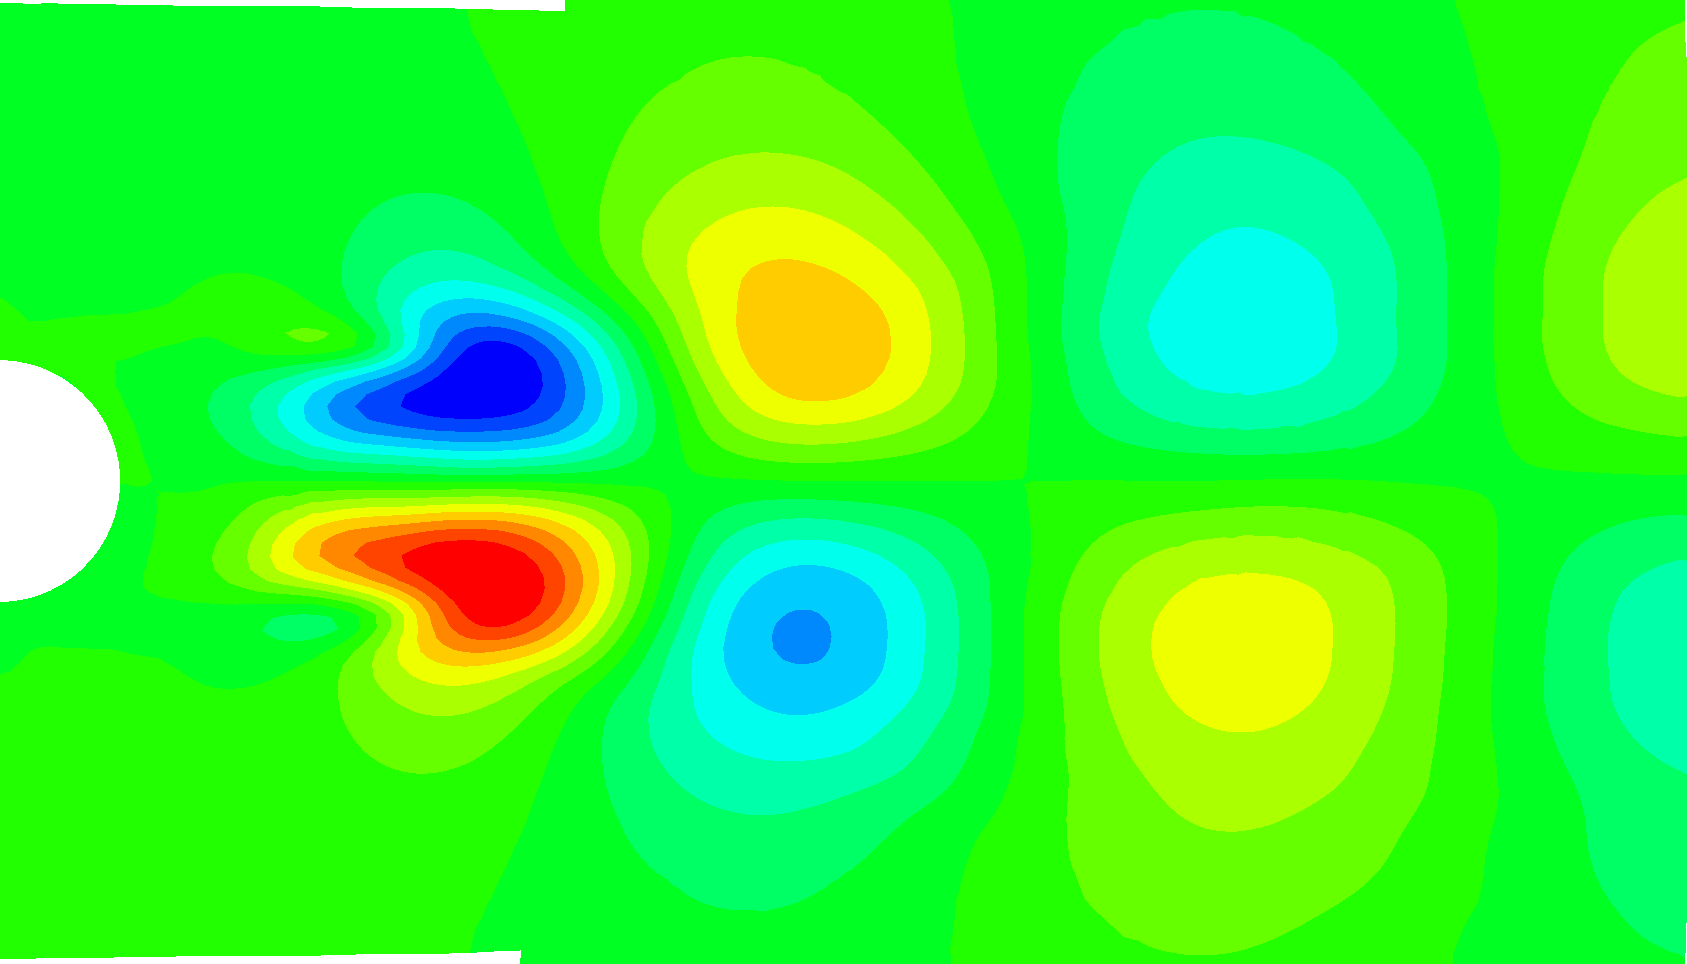
\includegraphics[trim = 0px 0px 0px 0px,clip,width = 0.39\textwidth]{\myImages/res/pom1top1numUx.png}}
	\begin{axis}[
		name = plot1,
		xlabel={$x_r$ [--]},
		ylabel={$y_r$ [--]},
		font = \scriptsize,
		xtick distance=1,ytick distance=1,
		width=\wd\mygraphic,
		height=\ht\mygraphic, %height= 5/3*0.5
		enlargelimits=false,
		scale only axis=true,
		tick align=outside,
		ytick pos=left,
		xtick pos=top,
		% x label style = {at={(axis description cs:3.5,2.5)}},
		x label style = {at={(axis cs:3.5,2.7)}},
		y label style = {at={(axis cs:-1,0)}},
		line width = 1.7pt
		]
		\addplot graphics[xmin=0, xmax=7, ymin=-2, ymax=2,includegraphics={trim = 0px 0px 0px 0px,clip}] {\myImages/res/pom1top1numUx.png};
		\fill [white] (axis cs:0.001,-1.997) rectangle (axis cs:0.5,1.997);
		\fill [black!70](axis cs:0,0) circle [radius=0.5];
		\node at (axis cs:0.22,1.7) {\scriptsize{a)}};
		% \draw [black,dashdotted,line width = 1.3pt] (axis cs:0,0) -- (axis cs:7,0);
		% \node at (axis cs:6.5,1.7) {\scriptsize{PIV}};
		% \node at (axis cs:6.5,-1.7) {\scriptsize{CFD}};
	\end{axis}

	\node [name = osaPsix,anchor = north,at={(plot1.south)},yshift=-0.1cm] {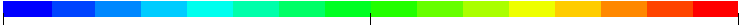
\includegraphics[width=0.39\textwidth]{\myImages/res/psi1_x_scale.png}};
	\node [name = psi0, anchor = north,at={(osaPsix.south)},yshift=0.2cm] {\scriptsize{0}};
	\node [name = psi, anchor = north,at={(psi0.south)},yshift=0.1cm] {\scriptsize{$\bm{\psi}_{1,x},\,_{\mathrm{r}}\bm{\psi}_{1,x}$}};
	\node [name = psiM05, anchor = north west,at={(osaPsix.south west)},yshift=0.2cm] {\scriptsize{negative}};
	\node [name = psiM05, anchor = north east,at={(osaPsix.south east)},yshift=0.2cm] {\scriptsize{positive}};

	% \node [name = psiM05, anchor = center,at={(psi0.center)},xshift=-1.2cm] {positive}};

	\savebox\mygraphic{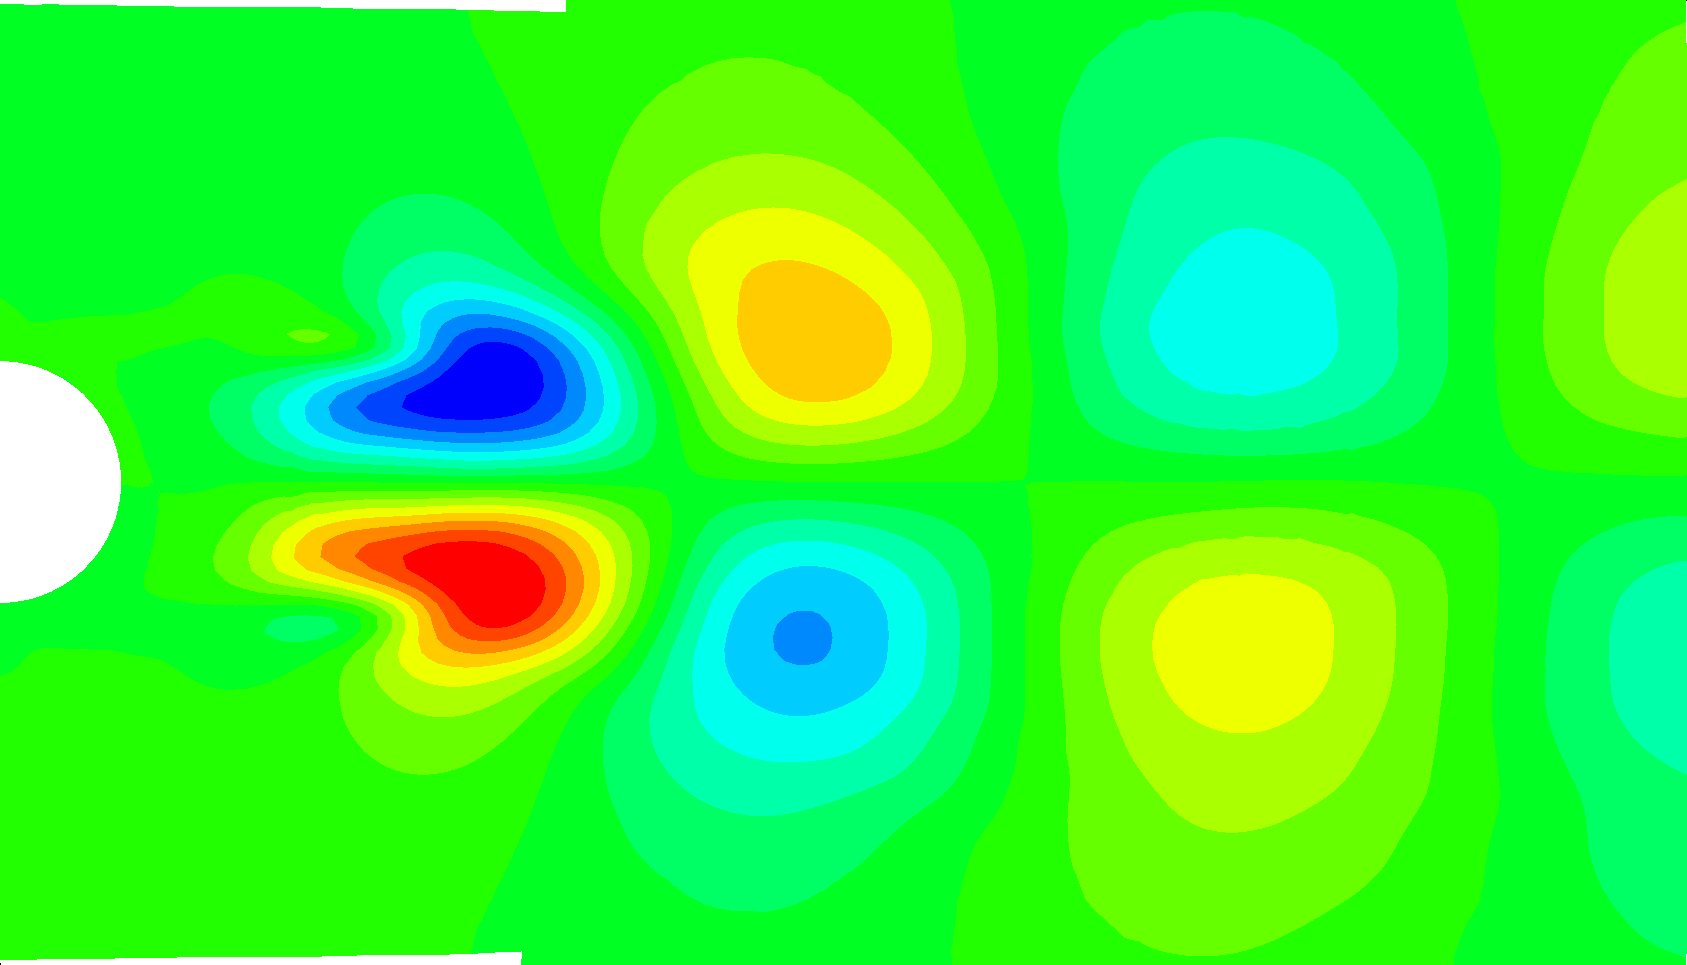
\includegraphics[trim = 0px 0px 0px 0px,clip,width = 0.39\textwidth]{\myImages/res/pom1top1numRNDpodUx.png}}
	\begin{axis}[
		name = plot2,
		anchor = north,
		at = {(psi.south)},
		yshift = -0.18cm,
		xlabel={$x_r$ [--]},
		ylabel={$y_r$ [--]},
		font = \scriptsize,
		xtick distance=1,ytick distance=1,
		x label style = {at={(axis cs:3.5,-2.7)}},
		y label style = {at={(axis cs:-1,0)}},
		width=\wd\mygraphic,
		height=\ht\mygraphic, %height= 5/3*0.5
		enlargelimits=false,
		scale only axis=true,
		ytick pos=left,
		xtick pos=bottom,
		tick align=outside,
		line width = 1.7pt
		]
		\addplot graphics[xmin=0, xmax=7, ymin=-2, ymax=2,includegraphics={trim = 0px 0px 0px 0px,clip}] {\myImages/res/pom1top1numRNDpodUx.png};
		\fill [white] (axis cs:0.001,-1.997) rectangle (axis cs:0.5,1.997);
		\fill [black!70](axis cs:0,0) circle [radius=0.5];
		\node at (axis cs:0.22,1.7) {\scriptsize{c)}};
		% \draw [black,dashdotted,line width = 1.3pt] (axis cs:0,0) -- (axis cs:7,0);
		% \node [color=white] at (axis cs:6.5,1.7) {\scriptsize{PIV}};
		% \node [color=white] at (axis cs:6.5,-1.7) {\scriptsize{CFD}};
	\end{axis}

	\savebox\mygraphic{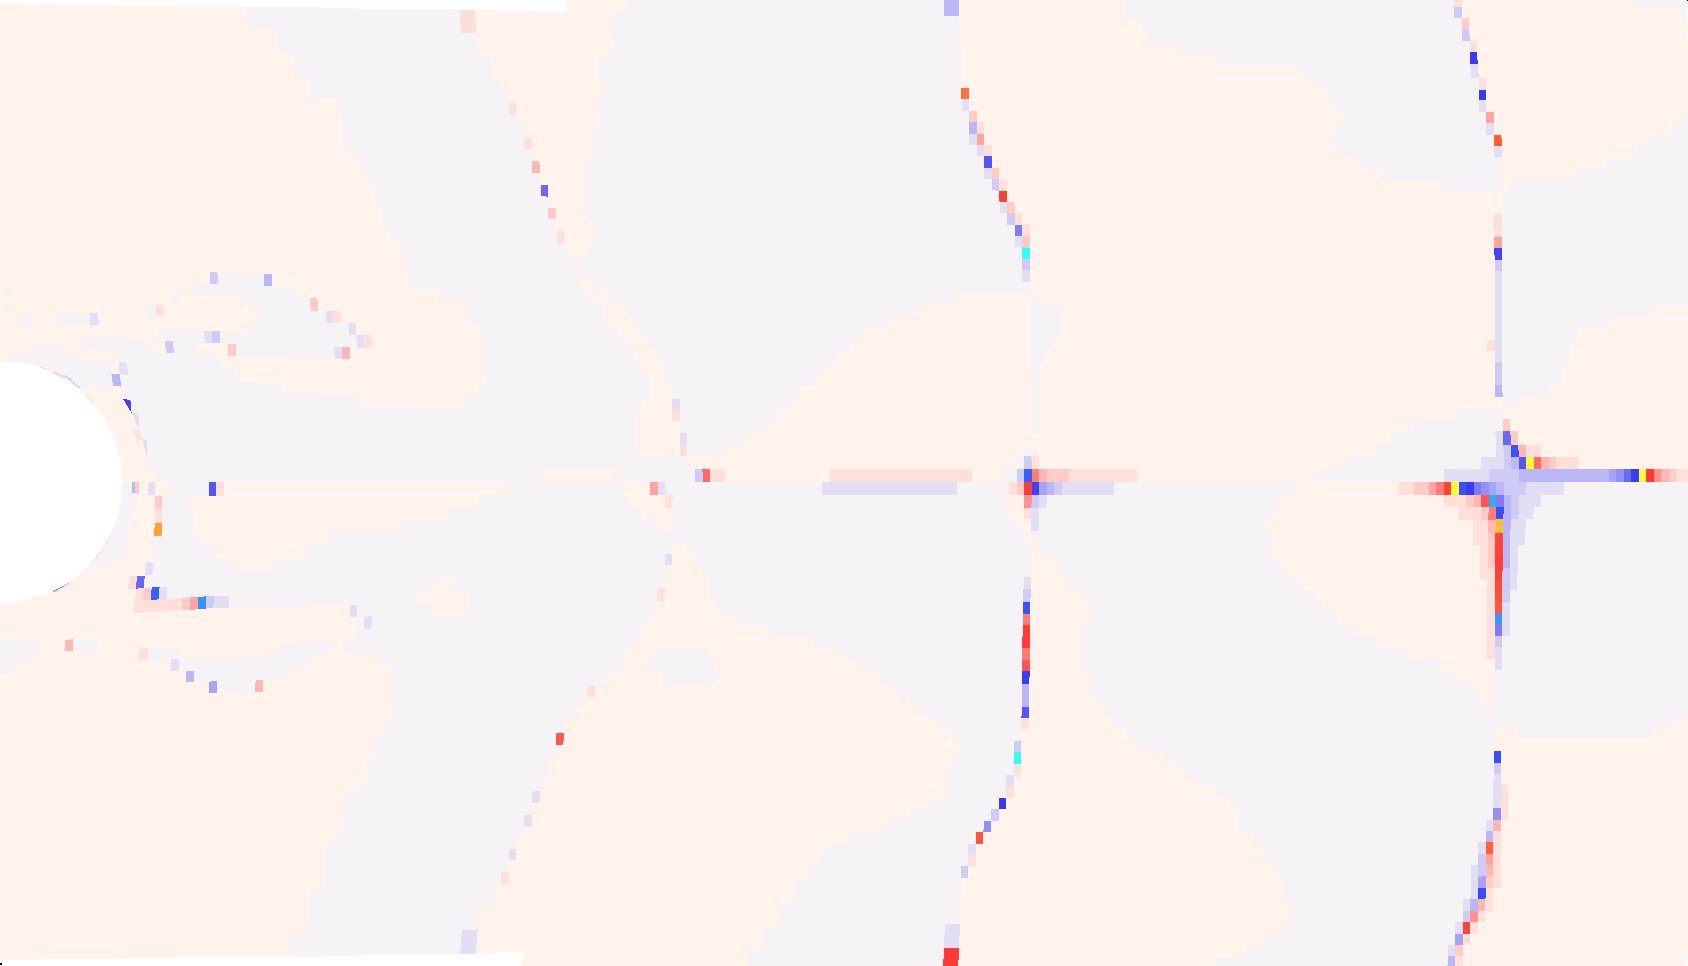
\includegraphics[trim = 0px 0px 0px 0px,clip,width = 0.39\textwidth]{\myImages/res/relDiffpodRNDpod.png}}
	\begin{axis}[
		name = plot3,
		xshift = 0.4cm,
		anchor = west,
		at = {(plot1.east)},
		xlabel={$x_r$ [--]},
		ylabel={$y_r$ [--]},
		font = \scriptsize,
		x label style = {at={(axis cs:3.5,2.7)}},
		y label style = {at={(axis cs:8,0)}},
		xtick distance=1,ytick distance=1,
		width=\wd\mygraphic,
		height=\ht\mygraphic, %height= 5/3*0.5
		enlargelimits=false,
		scale only axis=true,
		ytick pos=right,
		xtick pos=top,
		tick align=outside,
		line width = 1.7pt
		]
		\addplot graphics[xmin=0, xmax=7, ymin=-2, ymax=2,includegraphics={trim = 0px 0px 0px 0px,clip}] {\myImages/res/relDiffpodRNDpod.png};
		\fill [white] (axis cs:0.001,-1.997) rectangle (axis cs:0.5,1.997);
		\fill [black!70](axis cs:0,0) circle [radius=0.5];
		\node at (axis cs:0.22,1.7) {\scriptsize{b)}};
		% \draw [black,dashdotted,line width = 1.3pt] (axis cs:0,0) -- (axis cs:7,0);
		% \node [color=white] at (axis cs:6.5,1.7) {\scriptsize{PIV}};
		% \node [color=white] at (axis cs:6.5,-1.7) {\scriptsize{CFD}};
	\end{axis}
	
	\node [name = osaPsix,anchor = north,at={(plot3.south)},yshift=-0.1cm] {
\includegraphics[width=0.39\textwidth]{\myImages/res/relDiff_x_scale.png}};
	\node [name = psi0, anchor = north,at={(osaPsix.south)},yshift=0.2cm] {\scriptsize{0 \%}};
	\node [name = psi, anchor = north,at={(psi0.south)},yshift=0.1cm] {\scriptsize{$(\bm{\psi}_{1,x}-\,_{\mathrm{r}}\bm{\psi}_{1,x})/\bm{\psi}_{1,x}$}};
	\node [name = psiM05, anchor = north west,at={(osaPsix.south west)},yshift=0.2cm] {\scriptsize{-0.1 \%}};
	\node [name = psiM05, anchor = north east,at={(osaPsix.south east)},yshift=0.2cm] {\scriptsize{0.1 \%}};

	\begin{axis}[
		name = plot4,
		anchor = west,
		at = {(plot2.east)},
		xshift = 0.4cm,
		xlabel={mode number $j$},
		ylabel={$|\sigma_j - _{\mathrm{r}}\sigma_j|/\sigma_1$ [--]},
		font = \scriptsize,
		% xtick distance=1,ytick distance=1,
		width=\wd\mygraphic,
		height=\ht\mygraphic, %height= 5/3*0.5
		% x label style = {at={(axis cs:3.5,-2.7)}},
		% y label style = {at={(axis cs:-1,0)}},
		enlargelimits=false,
		scale only axis=true,
		ytick pos=right,
		xtick pos=bottom,
		ymode=log,
		line width = 0.85pt,
		xmax=30,
		xmin=0,
		ymin=1e-14,
		ymax=0.1,
		ytick={1e-1,1e-5,1e-10,1e-14}
		% tick align=outside,
		]
		\addplot [color = black,mark =triangle,only marks] table [x expr=\thisrow{x}+1, y expr = \thisrow{scaledWRTSigma1}]{\myGraphs/singValsData/singValsRND_U.dat};
		
		% \addplot [color = red,mark =x,only marks] table [x expr=\thisrow{x}+1, y expr = \thisrow{singVal}]{\myGraphs/singValsData/singValsRND_U.dat};
		% \addplot graphics[xmin=0, xmax=7, ymin=-2, ymax=2,includegraphics={trim = 0px 0px 0px 0px,clip}] {\myImages/res/relDiffpodRNDpod.png};
		% \fill [white] (axis cs:0.001,-1.997) rectangle (axis cs:0.5,1.997);
		% \fill [black!70](axis cs:0,0) circle [radius=0.5];
		% \draw [black,dashdotted,line width = 1.3pt] (axis cs:0,0) -- (axis cs:7,0);
		% \node [color=white] at (axis cs:6.5,1.7) {\scriptsize{PIV}};
		% \node [color=white] at (axis cs:6.5,-1.7) {\scriptsize{CFD}};
	\end{axis}
	\node[anchor=north west] at (plot4.north west) {\scriptsize{d)}};
\end{tikzpicture}

    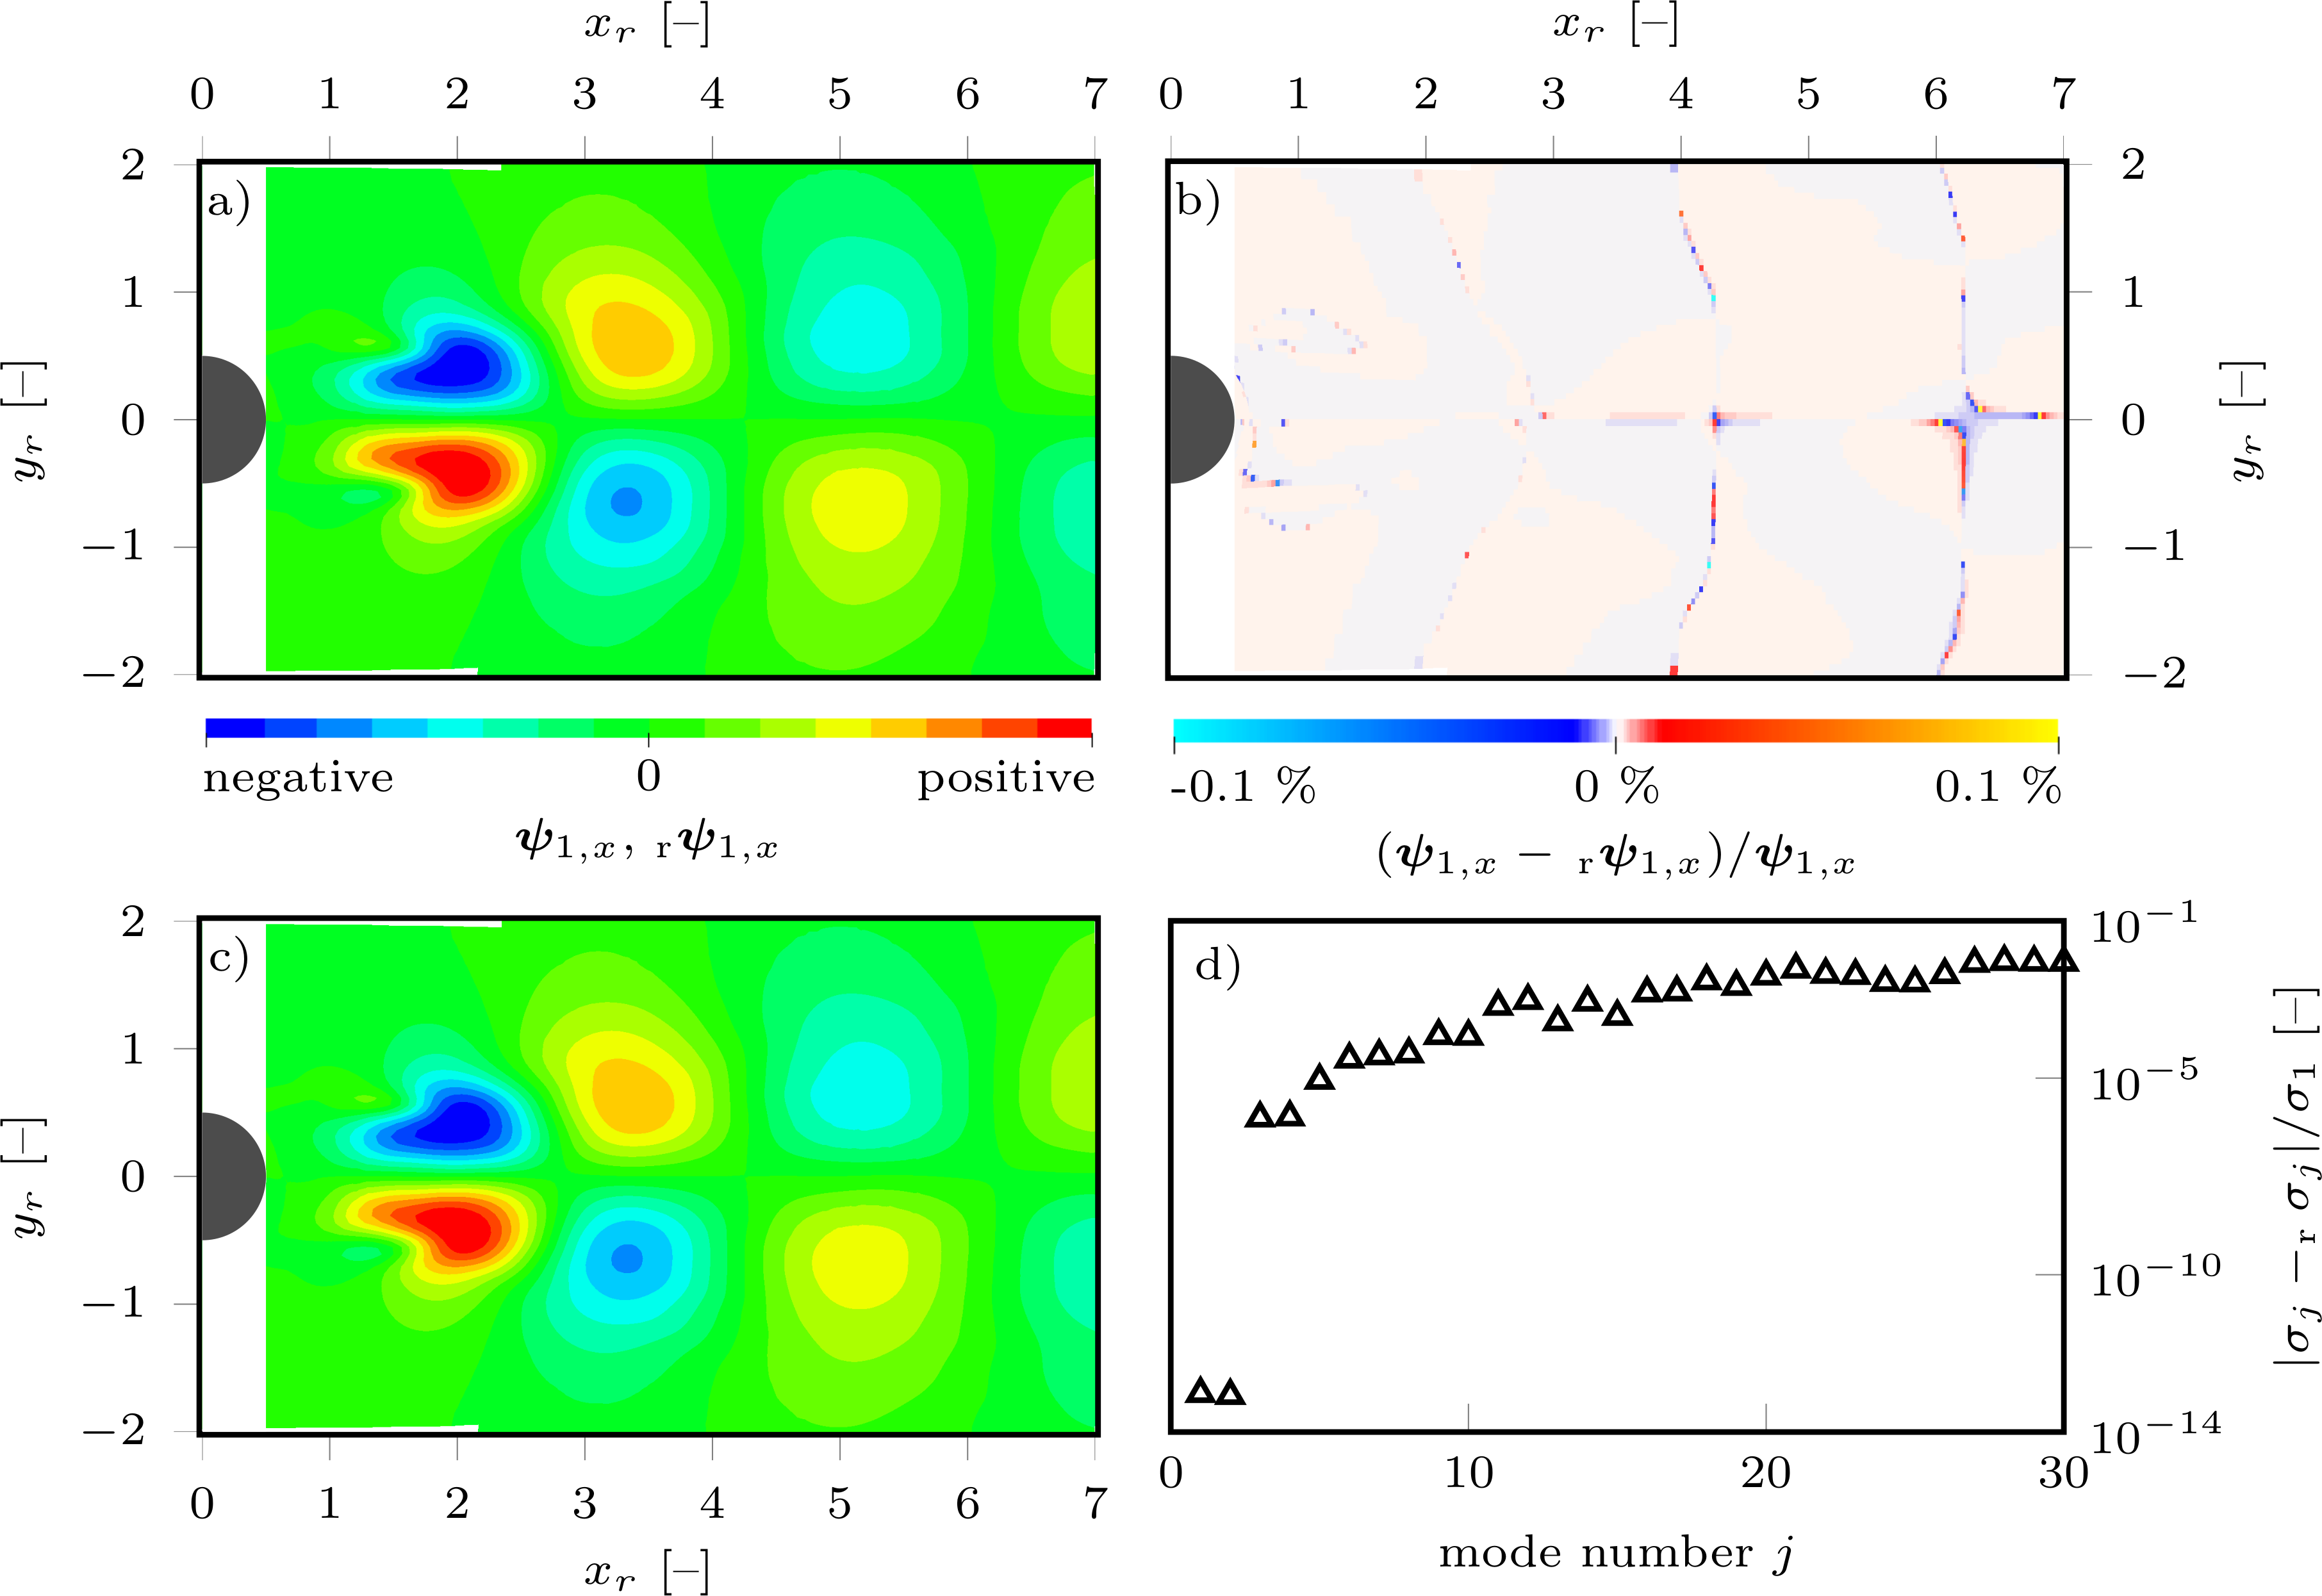
\includegraphics[width=0.98\textwidth]{02_images/00_export/figure4.png}
    \caption{POD and randomized POD (rPOD) results for simulated velocity field sampled on PoM1. (a) $\bm{\psi}_{1,x}$ computed via POD, (b) relative difference between the POD and rPOD toposes, (c) $_{\mathrm{r}}\bm{\psi}_{1,x}$ computed via rPOD, (d) relative difference between the first 30 POD and rPOD singular values.}
    \label{fig:podRandPODComp}
\end{figure}
In Figures~\ref{fig:podRandPODComp}a and~\ref{fig:podRandPODComp}c, we show the most energetic modes obtained via POD and randomized POD (rPOD) analysis of the simulated velocity data on PoM1, respectively. In Figure~\ref{fig:podRandPODComp}b, the relative error between the two datasets is depicted. Finally, note that the randomized POD variant was performed with $\ell = 30$. In Figure~\ref{fig:podRandPODComp}d, we compare the $\ell$ singular values $\sigma_{\ell}$ obtained via the standard and the randomized POD variant. Altogether, the data depicted in Figure~\ref{fig:podRandPODComp} show that from the point of view of the simulated system analysis, there is no perceivable difference between POD and rPOD.
